\documentclass[12pt, letterpaper]{article}
\usepackage[dvipsnames]{xcolor}

\usepackage{tikz}

\usepackage{fontspec} % used to import Calibri
\usepackage{anyfontsize} % used to adjust font size

\newfontfamily{\calibri}{Calibri}

\newcommand{\hOne}{
   \calibri
   \color{Blue}%
   \fontsize{14}{14}\selectfont%
}

\begin{document}

\hOne This is some text with your formatting. \[\sup{A}\]



\begin{center}
   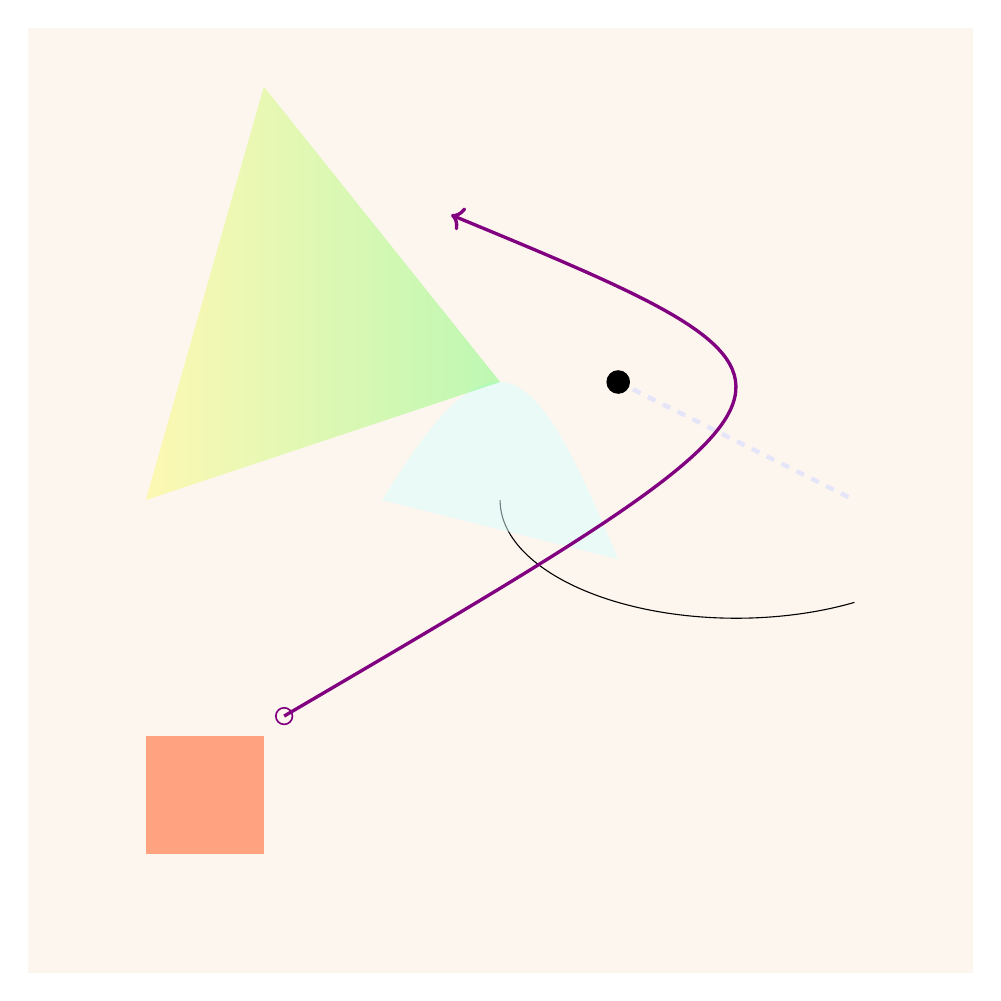
\begin{tikzpicture}[scale=1.5]
      \usetikzlibrary{arrows.meta}
      \tikzstyle help lines=[color=Lavender, ultra thick, dashed];
      
      \fill[Apricot!90!gray!10!White] (-5, -5) rectangle (3, 3);
      \clip (-5, -5) rectangle (3, 3); %another thing you can do apparently

      \draw[style=help lines] (0, 0) -- (2, -1);
      \fill (0, 0) circle (1mm);
      \draw (-1, -1) arc (180:300:2 and 1);

      \fill[Cyan!15, opacity=0.5] (-2, -1) sin (-1, 0) cos 
                                          (0, -1.5) -- cycle;
      
      \fill[OrangeRed!50] (-4, -4) -- (-3, -4) -- (-3, -3) -- (-4, -3)
         -- cycle;
      
      \shade[left color=yellow, right color=green, opacity=0.25]
         (-4, -1) -- (-3, 2.5) -- (-1, 0) -- cycle;

      %polar coordinates
      \draw[color=Purple, semithick] (225:4cm) circle (2pt);
      \draw[color=Purple, -To, very thick] (225:4cm) .. controls (0:2cm) .. (135:2cm);


   \end{tikzpicture}

\end{center}

\end{document}